\subsubsection{Language}
	Quickly, at the beginning of the project, we choose to use C++ to code our software. This is for simple reasons, C++ permits to create fast softwares so it's more indicate than Java to create an efficient algorithm.  Moreover it has several complete graphical libraries, like Qt or sfml, so it's easy to create the graphical interface that we need for the project.

\subsubsection{Software}
	We fixed the choice of the software solutions we will use to develop the project. The coding  will be realized on Microsoft visual studio 2013, and the version manager will be git. This two software are very used in the industry so we have to be familiar with them.
For the bibliography we will use Zotero, it permit the creation of .bib the bibliographic format use by LaTeX that we will used to write our reports.

\subsubsection{Grid5000}
	Grid5000 is a cluster of computers shared between many sites in France, it links a lot of computer of different centers of research, whose the IRISA. Some of this machines have, in addition of a good CPU, a NVIDIA Tesla GPU that could be use to parallelize the MCTS. Of Course use this cluster will require some specific parallelization that we will present in the next part.

\subsubsection{Parallelization}

\paragraph{Multi cores parrelization}\mbox{}\\\mbox{}\\
	OpenMp is a very simple and efficient parallelization language. It consists in some pre-compilation instructions, with only a few lines it permits to obtains a parallel version of our algorithm. But it isn't exempt of default, in fact, as you can see on the next illustration, it use a large part of shared memory, it allows a quick and efficient communication between the different threads but it's not designed for using a cluster of computers, because the memory access will be too long if this memory is used by two computers which are far away. But like we will see after, there is a method to avoid this problem.
\begin{figure}[!h] 
\centerline{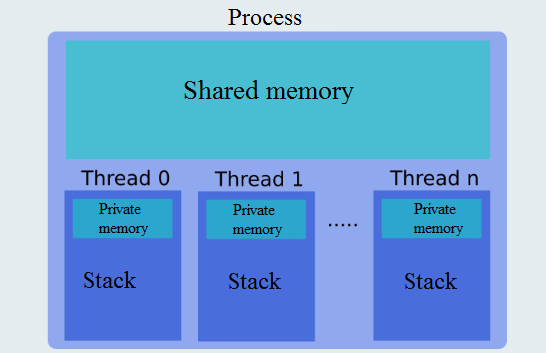
\includegraphics[scale=0.50]{3_Software_considered/MultithreadingMP_boost_Visual_MPI_5000_Zotero_Project_Baptiste/OpenMP}}
   \caption{\label{étiquette} OpenMp : memory management}
\end{figure}
\newpage
\paragraph{Computer parallelization}\mbox{}\\\mbox{}\\
	MPI is a more complex method of parallelization than openMp but it's more complete, in addition to use several cores on a single machine, we can also use MPI to designed our software to use a cluster of machines. As you can see on the illustration, it doesn't use shared memory, all the data of the threads are duplicate at their creation. It uses signals to permit the communication between the threads. One of its advantages is that it makes possible to use multiple computers, as the data are duplicated their isn't the problem of time to access the memory. But we have to pay attention to the cost of communication between the threads, if we use too much the signals we will lose all the time we can gain with the parallelization. It's very adapted for a tree parallelization, because with it we have just to duplicate the data at the beginning and return the result at the end of the assign time.

\begin{figure}[!h] 
\centerline{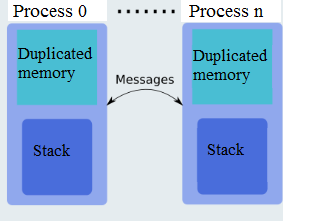
\includegraphics[scale=0.85]{3_Software_considered/MultithreadingMP_boost_Visual_MPI_5000_Zotero_Project_Baptiste/MPI}}
   \caption{\label{étiquette} MPI : memory management}
\end{figure}


\paragraph{Hybrid parallelization}\mbox{}\\\mbox{}\\
	As we see openMp and MPI have each one their advantage and inconvenience, but we can reduce the problems by using both. That means that we can use MPI to dispatch the work onto the different computers and after use openMp to divide it on the different threads of each machine. This can permit to use together multiples parallelization strategy like tree between the machine and leaf or root on each machine. Also it reduce the manual treatment that we have to define in the code to manage the threads. It means too that we reduce the threads interaction, so we kept a maximum of the parallel code.

\paragraph{Boost Library}\mbox{}\\\mbox{}\\
	Boost is a classical library of C++ which permits, amongst other things, the management of threads, basically we can use it only for one computer but it also contains a socket handling which should easily permit a parallelization between several machines. The library seems to be simple to use and complete. Also it holds tools for Graph modelisation that can improve a lot the efficiency of our algorithms.

\paragraph{GPU implementation}\mbox{}\\\mbox{}\\
	During our research we heard about using the GPU to improve the MCTS algorithms efficiency, as Kamil Rocki said in his thesis /cite{GPU-CPU parallelization} one GPU's performance is equivalent to 50 CPU threads. But this implementation has some defaults, in fact the Gpu possess very few cache memory, so if the data model is too big the parallelization will be inefficient. Also the trees that it creates will be less deep than those of a CPU, but when a CPU can develop 2 branches a GPU will develop hundreds branches simultaneously. Another thing we have to know is that a GPU can switch to another thread immediately without any cost of context switching. 
	Grid5000 has NVIDIA GPU so one of our possibility is to use hybrid as I describe previously by using MPI (or boost library) and openAcc (an equivalent of openMp which allows to use GPU) or CUBA (a framework for GPU parallelization develop by NVIDIA). In this way we should be able to develop greats trees and have a better solution compare with using only CPU, even if the trees will be less deep.